\documentclass[12pt, aspectratio=169]{beamer}

\usetheme[progressbar=frametitle]{metropolis}
\usepackage{appendixnumberbeamer}

\usepackage{booktabs}
\usepackage[scale=2]{ccicons}

\usepackage{pgfplots}
\usepgfplotslibrary{dateplot}

\usepackage{xspace}
\newcommand{\themename}{\textbf{\textsc{metropolis}}\xspace}

\usepackage{amsmath}
\usepackage{pgfplotstable}

\usetikzlibrary{positioning}
\usetikzlibrary{shapes.misc,shapes}
\usetikzlibrary{decorations.pathreplacing}

\definecolor{blue}{RGB}{0,91,130}% Diagram color blue % 100%
\definecolor{lightblue}{RGB}{110,159,189}% Diagram color blue % 50%
\definecolor{red}{RGB}{185,70,60}% Diagram color red % 100%
\definecolor{lightred}{RGB}{198,141,132}% Diagram color red % 70%
\definecolor{green}{RGB}{50,120,50}% Diagram color green % 100%
\definecolor{lightgreen}{RGB}{164,181,153}% Diagram color green % 70%
\definecolor{orange}{HTML}{D7AA50}
\definecolor{purple}{HTML}{7A68A6}

\usetikzlibrary{calc}
\usetikzlibrary{fit}
\usetikzlibrary{positioning}
\usetikzlibrary{shapes.misc,shapes}
\usetikzlibrary{decorations.pathreplacing}


%%%%%%%%%%%%%%%%%% START PRESENTATION %%%%%%%%%%%%%%%%%%%%%%%%%%%%%%%%%%%%%%
\title{Deep On-Chip Learning on BrainScaleS-2}
\subtitle{MFP Talk}
% \date{\today}
\date{}
\author{Simeon Kanya}
\institute{Kirchhoff-Institute for Physics - Electronic Vision(s) Group}
% \titlegraphic{\hfill\includegraphics[height=1.5cm]{logo.pdf}}

\begin{document}

\maketitle
%%%%%%%%%%%%%%%%%%%%%%%%%%%%%% INTRODUCTION %%%%%%%%%%%%%%%%%%%%%%%%%%%%%%%%
\section[Intro]{Introduction}

\begin{frame}{Deep Learning}
  \begin{figure}[!htb]
    	\minipage{0.6\textwidth}
	        \textbf{Forward pass:} output values of each node in the network is evaluated.\\
            
            \textbf{Backward pass:} perform gradient decent on a \textbf{loss function} and thus find a set of model parameters (e.g. weights) which minimizes the loss.\\
	   
            \endminipage\hfill
      	\minipage{0.4\textwidth}
        \begin{figure}
           \scalebox{1.3}{\pgfmathsetseed{123456789}%
\tikzset{expressed/.style={-stealth,shorten <=4pt,shorten >=6pt,ultra thick}}%
\tikzset{potential/.style={-stealth,shorten <=4pt,shorten >=6pt,very thick,dotted}}%
\usetikzlibrary{calc}
%

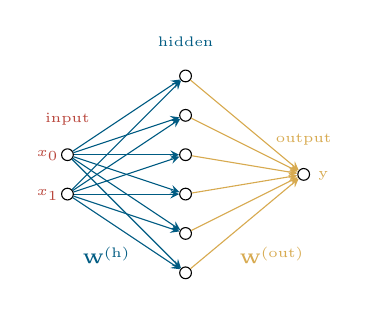
\begin{tikzpicture}{scale=2.0}
	\foreach \i in {0,...,1} \node[draw,circle,inner sep=1.5pt] (input\i) at (0,\the\numexpr0.5*\i+1.0+0.75) {};
	\foreach \i in {0,...,5} \node[draw,circle,inner sep=1.5pt] (hidden\i) at (1.5,\the\numexpr0.5*\i+0.75) {};
    \foreach \i in {0,...,0} \node[draw,circle,inner sep=1.5pt] (output\i) at (3.0,\the\numexpr0.5*\i+1.25+.75) {};

    % connectors input -> hidden
	\foreach \i in {0,...,1}
		\foreach \j in {0,...,5} \draw[-stealth,blue!100!white] (input\i) -- (hidden\j);

    % connectors hidden -> output
	\foreach \i in {0,...,5}
		\foreach \j in {0,...,0} \draw[-stealth,orange!100!white] (hidden\i) -- (output\j);

    % labels
	\draw (input1) ++ (0.0,0.25) node[red,above] {\tiny input};
	\draw (input0) ++ (-0.25,-0.20) node[red!100!white,above] {\tiny $x_1$};
	\draw (input1) ++ (-0.25,-0.20) node[red!100!white,above] {\tiny $x_0$};
	\draw (hidden5) ++ (0.0,0.25) node[blue,above] {\tiny hidden};
	\draw (output0) ++ (0.0,0.25) node[orange,above] {\tiny output};
	\draw (output0) ++ (0.25,-0.20) node[orange,above] {\tiny y};		

	% weight labels
	\draw (input0) ++ (0.5,-1.0) node[blue!100!white,above] {\tiny $\textbf{W}^{\text{(h)}}$};
	\draw (hidden0) ++ (1.1,0) node[orange!100!white,above] {\tiny $\textbf{W}^{\text{(out)}}$};	
	 \node[draw,color=white] (dummy) at (0,0.5) {};
\end{tikzpicture}
}
            \label{neural network}
        \end{figure}
        \endminipage\hfill
    \end{figure}
\end{frame}

% Details on components of network
\begin{frame}{Forward Pass}
  \begin{figure}[!htb]
    	\minipage{0.6\textwidth}
            The \textbf{activation} $\vec{a}$ of a neuron
            \begin{equation}
                \vec{a} = W \vec{x} + \vec{b}.
            \end{equation}
            
            The \textbf{transfer function} $\phi$ yields an \textbf{output} $\vec{y}$
            \begin{equation}
                \vec{y} = \phi(\vec{a}).
            \end{equation}
            \endminipage\hfill
      	\minipage{0.4\textwidth}
      	\vspace{20pt}
      	\centering
        \begin{figure}
           \scalebox{1.5}{\pgfmathsetseed{123456789}%
\tikzset{expressed/.style={-stealth,shorten <=4pt,shorten >=6pt,ultra thick}}%
\tikzset{potential/.style={-stealth,shorten <=4pt,shorten >=6pt,very thick,dotted}}%
\usetikzlibrary{calc}

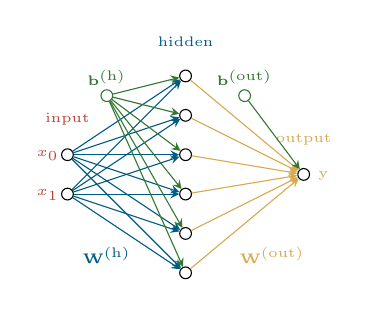
\begin{tikzpicture}
	\foreach \i in {0,...,1} \node[draw,circle,inner sep=1.5pt] (input\i) at (0,\the\numexpr0.5*\i+1.0+0.75) {};
	\foreach \i in {0,...,5} \node[draw,circle,inner sep=1.5pt] (hidden\i) at (1.5,\the\numexpr0.5*\i+0.75) {};
    \foreach \i in {0,...,0} \node[draw,circle,inner sep=1.5pt] (output\i) at (3.0,\the\numexpr0.5*\i+1.25+.75) {};

    % connectors input -> hidden
	\foreach \i in {0,...,1}
		\foreach \j in {0,...,5} \draw[-stealth,blue!100!white] (input\i) -- (hidden\j);

    % connectors hidden -> output
	\foreach \i in {0,...,5}
		\foreach \j in {0,...,0} \draw[-stealth,orange!100!white] (hidden\i) -- (output\j);

    % labels
	\draw (input1) ++ (0.0,0.25) node[red,above] {\tiny input};
	\draw (input0) ++ (-0.25,-0.20) node[red!100!white,above] {\tiny $x_1$};
	\draw (input1) ++ (-0.25,-0.20) node[red!100!white,above] {\tiny $x_0$};
	\draw (hidden5) ++ (0.0,0.25) node[blue,above] {\tiny hidden};
	\draw (output0) ++ (0.0,0.25) node[orange,above] {\tiny output};
	\draw (output0) ++ (0.25,-0.20) node[orange,above] {\tiny y};	
    
    % bias nodes
    \node[color=green,draw,circle,inner sep=1.5pt] (bias1) at (0.5,5*0.5+0.5) {};
	\draw (bias1) ++ (0.0,0.0) node[green,above] {\tiny $\textbf{b}^{\text{(h)}}$};
	
    \node[color=green,draw,circle,inner sep=1.5pt] (bias2) at (2.25,5*0.5+0.5) {};
	\draw (bias2) ++ (0.0,0.0) node[green,above] {\tiny $\textbf{b}^{\text{(out)}}$};

    % bias connectors
	\foreach \i in {0,...,5} \draw[-stealth,green!100!white] (bias1) -- (hidden\i);
	\draw[-stealth,green!100!white] (bias2) -- (output0);
    
	% weight labels
	\draw (input0) ++ (0.5,-1.0) node[blue!100!white,above] {\tiny $\textbf{W}^{\text{(h)}}$};
	\draw (hidden0) ++ (1.1,0) node[orange!100!white,above] {\tiny $\textbf{W}^{\text{(out)}}$};
	
	 \node[draw,color=white] (dummy) at (0,0.5) {};
\end{tikzpicture}}
            \label{neural network}
        \end{figure}
        \endminipage\hfill
    \end{figure}
\end{frame}

% Gradient Descent on components of network
\begin{frame}{Backward Pass and Gradient Descent}
Gradient descent is performed on the \textbf{loss function} $\mathcal{L}$. Given a \textbf{learning rate} $\eta$ the parameters (e.g. weight) update accordingly:\\
\begin{align*}
   \text{output:} \quad \delta W =& - \eta \frac{\partial \mathcal{L}}{\partial W} 
            = - \eta \;
            \underbrace{\frac{\partial\mathcal{L}}{\partial \vec{y}} \;
                        \frac{\partial \vec{y}}{\partial \vec{a} }}_{=\vec{e}\, \text{(error)}} \;
              \frac{\partial \vec{a}}{\partial W}
            = - \eta \, (\vec{e} \cdot \vec{x}^T)\\
            \\ 
   \text{hidden:} \quad \delta W =& - \eta \;
                                (W^T \cdot \vec{e}) \;
                                \nabla \phi(\vec{a}) \;
                                \vec{x}^T
\end{align*}
\end{frame}

\begin{frame}{Backward Pass and Gradient Descent}
Gradient descent is performed on the \textbf{loss function} $\mathcal{L}$. Given a \textbf{learning rate} $\eta$ the parameters (e.g. weight) update accordingly:\\
\begin{align*}
   \text{output:} \quad \delta W =& - \eta \frac{\partial \mathcal{L}}{\partial W} 
            = - \eta \;
            \underbrace{\frac{\partial\mathcal{L}}{\partial \vec{y}} \;
                        \frac{\partial \vec{y}}{\partial \vec{a} }}_{=\vec{e}\; \text{(error)}} \;
              \frac{\partial \vec{a}}{\partial W}
            = - \eta \, (\vec{e} \cdot \vec{x}^T)\\
            \\ 
   \text{hidden:} \quad \delta W =& - \eta \;
                                (W^T \cdot \vec{e}) \;
                                \nabla \phi(\vec{a}) \;
                                \vec{x}^T\\
   \text{feedback alignment:} \quad \delta W =& - \eta \;
                                (B \cdot \vec{e}) \;
                                \nabla \phi(\vec{a}) \;
                                \vec{x}^T\;\\
    \text{with } B \text{ being random matrix}
\end{align*}
\end{frame}

\section[Implementation on DLSv2]{Implementation on DLSv2}
% How is the activation of an hidden layer working
% Neuron (Vmem + Noise)
\begin{frame}{Membrane Potential and Noise}
    \begin{figure}[!htb]    	
        \minipage{0.5\textwidth}
        \centering
            \begin{figure}
               \scalebox{1.75}{\pgfmathsetseed{123456789}%
\tikzset{expressed/.style={-stealth,shorten <=4pt,shorten >=6pt,ultra thick}}%
\tikzset{potential/.style={-stealth,shorten <=4pt,shorten >=6pt,very thick,dotted}}%
\usetikzlibrary{calc}

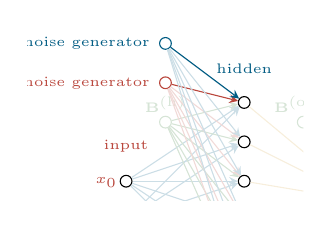
\begin{tikzpicture}
\clip (-1.25,2) rectangle + (3.5,2.2);
	\foreach \i in {0,...,1} \node[draw,circle,inner sep=1.5pt] (input\i) at (0,\the\numexpr0.5*\i+1.0+0.75) {};
	\foreach \i in {0,...,5} \node[draw,circle,inner sep=1.5pt] (hidden\i) at (1.5,\the\numexpr0.5*\i+0.75) {};
    \foreach \i in {0,...,0} \node[draw,circle,inner sep=1.5pt] (output\i) at (3.0,\the\numexpr0.5*\i+1.25+.75) {};

    % connectors input -> hidden
	\foreach \i in {0,...,1}
		\foreach \j in {0,...,5} \draw[-stealth,blue!20!white] (input\i) -- (hidden\j);

    % connectors hidden -> output
	\foreach \i in {0,...,5}
		\foreach \j in {0,...,0} \draw[-stealth,orange!20!white] (hidden\i) -- (output\j);

    % labels
	\draw (input1) ++ (0.0,0.25) node[red,above] {\tiny input};
	\draw (input0) ++ (-0.25,-0.20) node[red!100!white,above] {\tiny $x_1$};
	\draw (input1) ++ (-0.25,-0.20) node[red!100!white,above] {\tiny $x_0$};
	\draw (hidden5) ++ (0.0,0.25) node[blue,above] {\tiny hidden};
	\draw (output0) ++ (0.0,0.25) node[orange,above] {\tiny output};
	\draw (output0) ++ (0.25,-0.20) node[orange,above] {\tiny y};		
    
    % bias nodes
    \node[color=green!20!white,draw,circle,inner sep=1.5pt] (bias1) at (0.5,5*0.5+0.5) {};
	\draw (bias1) ++ (0.0,0.0) node[green!20!white,above] {\tiny $\textbf{B}^{\text{(h)}}$};
	
    \node[color=green!20!white,draw,circle,inner sep=1.5pt] (bias2) at (2.25,5*0.5+0.5) {};
	\draw (bias2) ++ (0.0,0.0) node[green!20!white,above] {\tiny $\textbf{B}^{\text{(out)}}$};

    % bias connectors
	\foreach \i in {0,...,5} \draw[-stealth,green!20!white] (bias1) -- (hidden\i);
	\draw[-stealth,green!20!white] (bias2) -- (output0);
    
	% weight labels
	\draw (input0) ++ (0.5,-1.0) node[blue!20!white,above] {\tiny $\textbf{W}^{\text{(h)}}$};
	\draw (hidden0) ++ (1.1,0) node[orange!20!white,above] {\tiny $\textbf{W}^{\text{(out)}}$};

    % noise generators
    \node[color=red!100!white,draw,circle,inner sep=1.5pt] (noise1) at (0.5,5*0.5+0.5+0.5) {};
	\draw (noise1) ++ (-1.,-0.2) node[red!100!white,above] {\tiny noise generator};
    \node[color=blue!100!white,draw,circle,inner sep=1.5pt] (noise2) at (0.5,5*0.5+0.5+1.0) {};
	\draw (noise2) ++ (-1.0,-0.2) node[blue!100!white,above] {\tiny noise generator};
    
    % noise connectors
    \draw[-stealth,red!100!white] (noise1) -- (hidden5);
    \draw[-stealth,blue!100!white] (noise2) -- (hidden5);
	\foreach \i in {0,...,4} \draw[-stealth,red!20!white] (noise1) -- (hidden\i);
	\foreach \i in {0,...,4} \draw[-stealth,blue!20!white] (noise2) -- (hidden\i);
	
	 \node[draw,color=white] (dummy) at (0,0.5) {};
\end{tikzpicture}}
                \label{neural network}
            \end{figure}
      	\endminipage\hfill
      	\minipage{0.5\textwidth}
        	\vspace{20pt}
      	    \centering
            \begin{figure}
                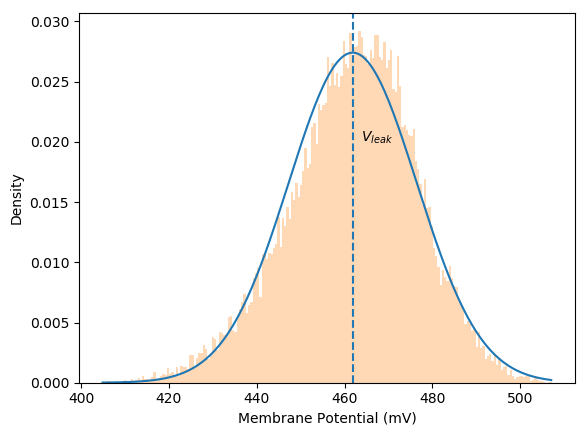
\includegraphics[scale=0.5]{activation_function_vmem_distr.png}
                \label{membrane_potential}
            \end{figure}
        \endminipage\hfill
    \end{figure}
\end{frame}

% Neuron + Threshold => spikes
\begin{frame}{Membrane Potential and Threshold}
    \begin{figure}[!htb]
    	\minipage{0.5\textwidth}
            \begin{itemize}
                \item membrane potential exceeds the threshold $\Rightarrow$ spiking
                \item fast time constants necessary
                \item $\delta V = V_{\text{leak}} - V_{\text{thres}}$
                \item transfer function $\phi$ depends on $\delta V$
            \end{itemize}
      	\endminipage\hfill
      	\minipage{0.5\textwidth}
      	    \centering
      	    \vspace{20pt}
            \begin{figure}
                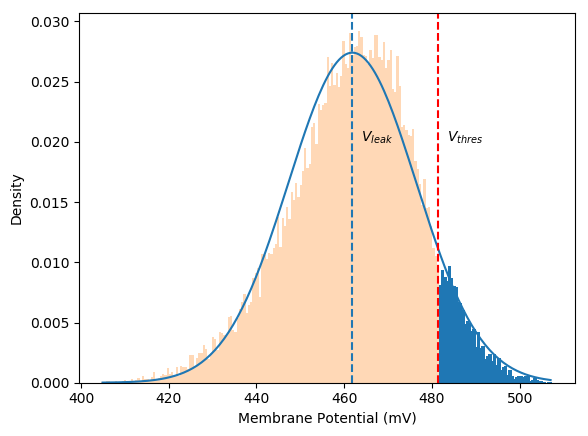
\includegraphics[scale=0.5]{activation_function_vmem_distr_with_thres.png}
                \label{membrane_potential}
            \end{figure}
        \endminipage\hfill
    \end{figure}
\end{frame}

% Neuron + input => move distr
\begin{frame}{Membrane Potential and Input}
    \begin{figure}[!htb]
    	\minipage{0.5\textwidth}
            \begin{itemize}
                \item excitatory input (Poisson spiketrain with $\sim 40 \text{kHz}$)
                \item inhibitory and excitatory noise (each $\sim 30 \text{kHz}$)
                \item weights: $w_{\text{input}} = 2 \times w_{\text{noise}}$
                \item inhibitory input for other direction
            \end{itemize}
      	\endminipage\hfill
      	\minipage{0.5\textwidth}
      	    \centering
      	    \vspace{20pt}
            \begin{figure}
            
                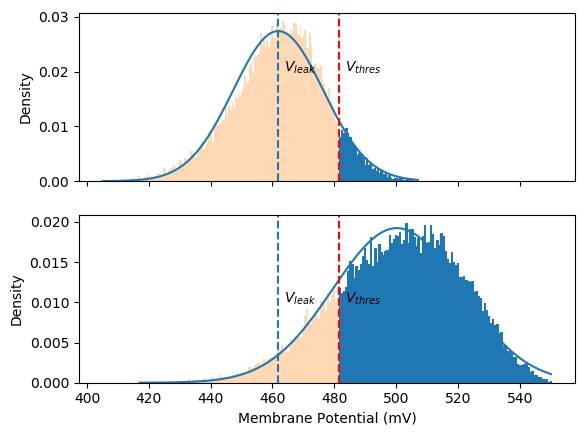
\includegraphics[scale=0.5]{activation_function_vmem_distr_with_input_with_thres.png}
                \label{membrane_potential}
            \end{figure}
        \endminipage\hfill
    \end{figure}
\end{frame}

\begin{frame}{Transfer Function on DLSv2}
    \centering
            \begin{figure}
                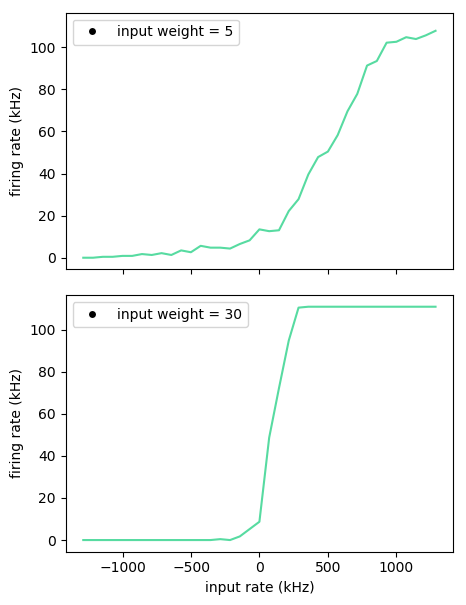
\includegraphics[scale=0.48]{uncalibrated_activation_function_input_single.png}
                \label{membrane_potential}
            \end{figure}
\end{frame}

\begin{frame}{Transfer Function on DLSv2}
    \centering
            \begin{figure}
                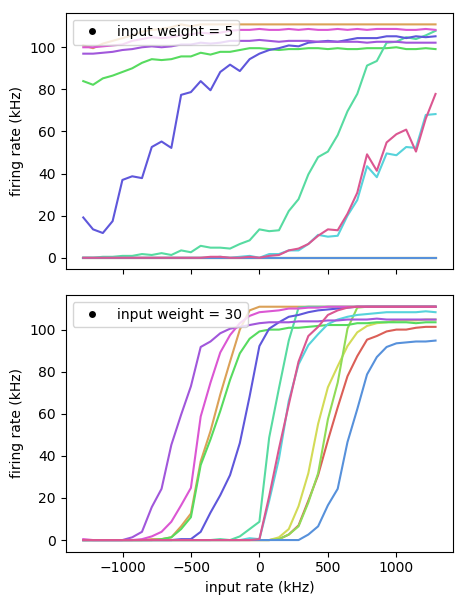
\includegraphics[scale=0.48]{uncalibrated_activation_function_input.png}
                \label{membrane_potential}
            \end{figure}
\end{frame}

\begin{frame}{Un-/Calibrated Transfer Functions}
    \begin{figure}[!htb]
    	\minipage{0.5\textwidth}
            \centering
            \textbf{uncalibrated}
            \begin{figure}
                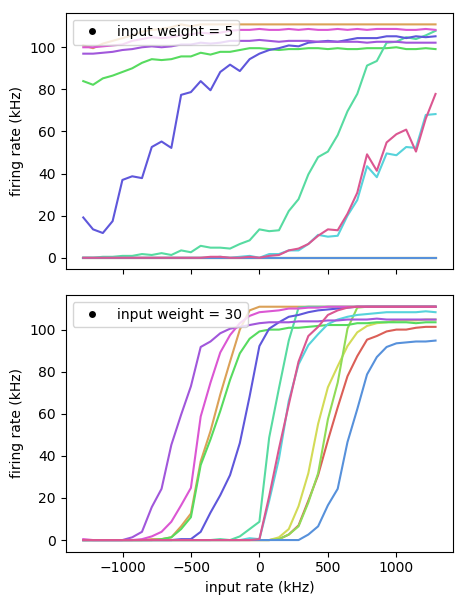
\includegraphics[scale=0.44]{uncalibrated_activation_function_input.png}
                \label{membrane_potential}
            \end{figure}
      	\endminipage\hfill
      	\minipage{0.5\textwidth}
            \centering
            \textbf{calibrated}
            \begin{figure}
                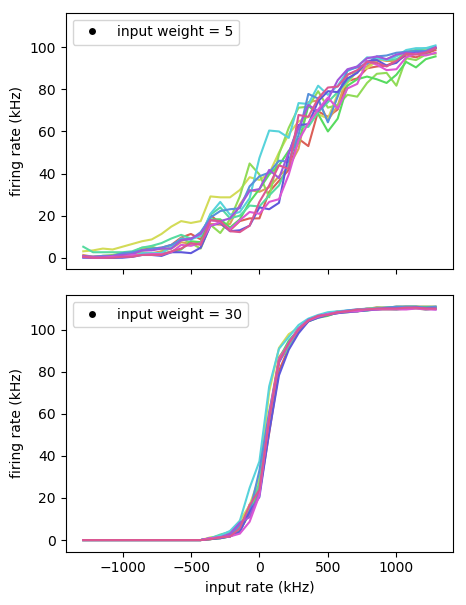
\includegraphics[scale=0.44]{calibrated_activation_function_input.png}
                \label{membrane_potential}
            \end{figure}
        \endminipage\hfill
    \end{figure}
\end{frame}

% What about Bias => move the threshold around
\begin{frame}{$V_{\text{thres}}$ as Bias}
    \begin{figure}[!htb]
    	\minipage{0.5\textwidth}
            \begin{itemize}
                \item moving $V_{\text{thres}}$ changes $\delta V$
                \item bias $b \propto \delta V $\\
                \item $b < 0 \Rightarrow $ fewer spikes $\Rightarrow$ shifted to the right
                
                \item conserves the working point of the membrane potential
            \end{itemize}
      	\endminipage\hfill
      	\minipage{0.5\textwidth}
            \centering
            \vspace{20pt}
            \begin{figure}
                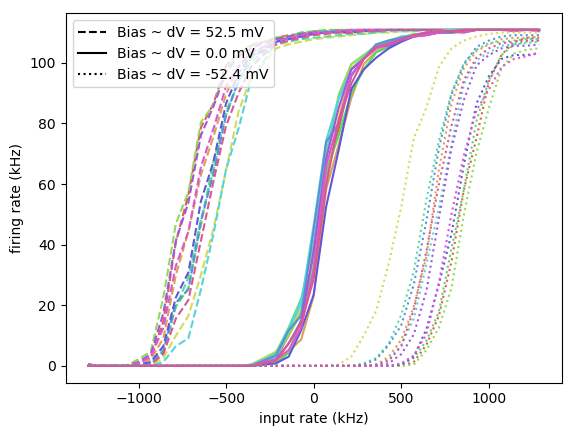
\includegraphics[scale=0.5]{bias_for_activation_function.png}
                \label{membrane_potential}
            \end{figure}
        \endminipage\hfill
    \end{figure}
\end{frame}

%%%%%%%%%%%%%%%%%%%%%%%%%%%%% LEARNING PROCESS %%%%%%%%%%%%%%%%%%%%%%%%%%%%
\section[Learning]{Deep Learning}
% What about Bias => move the threshold around
\begin{frame}{Learning Task: Circles}
    \begin{figure}[!htb]
    	\minipage{0.65\textwidth}
            \begin{itemize}
                \item feature plane: two inputs ("x" and "y")
                \item two classes:
                \begin{enumerate}
                    \item inner circle: \textbf{low} target rate $y^* = 32.6\, \text{kHz}$
                    \item outer circle: \textbf{high} target rate $y^* = 93.5\, \text{kHz}$
                \end{enumerate}
                \item find an appropriate decision-boundary
                \item on-Chip learning only
            \end{itemize}
      	\endminipage\hfill
      	\minipage{0.35\textwidth}
            \centering
            \begin{figure}
                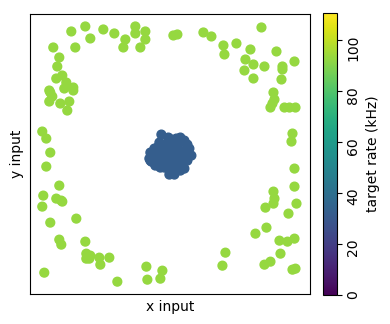
\includegraphics[scale=0.5]{targets.png}
                \label{membrane_potential}
            \end{figure}
        \endminipage\hfill
    \end{figure}
\end{frame}

\begin{frame}{On-Chip Experiment Design}
    \begin{figure}[!htb]
    	\minipage{0.6\textwidth}
    	    \textbf{Analog Core}
            \begin{itemize}
                \item $32$ LIF neurons
                \item $32 \times 32$ current based synapses
            \end{itemize}
        \textbf{PPU}
            \begin{itemize}
                \item experiment control
                \item noise and input generation
                \item update model parameters
            \end{itemize}
        
      	\endminipage\hfill
      	\minipage{0.4\textwidth}
      	\centering
      	
            \scalebox{.9}{\tikzset{block/.style={font={\sffamily\footnotesize},align=center}}%
\tikzset{box/.style={draw=black!90}}%
\tikzset{block label/.style={fill=white,font={\sffamily\footnotesize},inner sep=0.05cm}}%
\begin{tikzpicture}[
	baseline=(anc.south),
            font={\sffamily \small},
            scale=0.7,
            >=latex,
            transform shape,
	    line width=1.0\pgflinewidth,
	    anchor=center
        ]
        \pgfdeclarelayer{background layer}
        \pgfsetlayers{background layer,main}
        %\draw[use as bounding box,inner sep=0pt,draw=none] (-6.5,-3.0) rectangle ++(13,5.5);

	\node[block,box,minimum width=3.0cm,minimum height=2.0cm] (syn) at (0,0) {};
	\node[block,minimum width=3.0cm,minimum height=0.5cm,below=0.2cm of syn] (nrn) {};
	\node[block,box,minimum width=3.0cm,minimum height=0.5cm,below=0.1cm of nrn] (cm) {parameter storage};

	\node[block,minimum width=0.5cm,minimum height=2.0cm,left=0.05cm of syn] (drv) {};
	\node[block,minimum width=0.2cm,minimum height=2.0cm,left=0.05cm of drv] (padi) {};
	
	\node[block,box,minimum width=3.0cm,minimum height=0.3cm,above=0.1cm of syn] (cadc) {CADC};
	\node[block,box,minimum width=3.0cm,minimum height=0.5cm,above=0.2cm of cadc] (ppu) {PPU};

	% fitted analog core
	\node[anchor=north west,gray,rotate=90] (anc) at (cm.south east) {\scriptsize analog network core};
	\node[block,box,gray,dashed,fit={(padi) (cadc) (anc)},inner sep=0.1cm] (anc bound) {};

	% digital control and events
	\node[block,box,anchor=south east,minimum width=1.7cm,minimum height=0.8cm] (event)
		at ($(nrn.south west -| anc bound.west) + (-0.2,0.2)$) {Event \\ Handling};
	\node[block,box,anchor=south east,minimum width=2.2cm,minimum height=0.4cm] (link)
		at ($(anc bound.south west) - (0.2,0.0)$) {I/O};
	\node[block,box,anchor=north east,minimum width=1.7cm,minimum height=1.2cm] (mem)
		at ($(anc bound.north west) - (0.2,0.0)$) {Config.\\Memory\\Controllers};

	\foreach \x in {0,1,...,5} {
		\draw[] (nrn.south west) ++ (\x*0.5,0.0) ++ (0.25,0.25) circle (0.2cm);
		\draw[gray,latex-] (syn.south west) ++ (\x*0.5+0.25,-0.22) -- ++(0.0,2.22);
		
		\foreach \y in {0,1,...,3}
			\draw[gray] (syn.south west) ++ (\x*0.5+0.25,0.25+\y*0.5) circle (0.02cm);
	}

	\foreach \y in {0,1,...,3} {
		\draw[] (drv.south west) ++ (0.0,\y*0.5) ++ (0.1,0.05) -- ++(0.0,0.4) -- ++(0.3,-0.2) -- cycle;
		\draw[gray] (syn.south west) ++ (-0.1,\y*0.5+0.25) -- ++(3.0,0.0) -- ++(0.1,0.0);
	}

	% arrows
	\draw ($(event.east |- drv.south west) + (0.0,0.25)$) -- ($(drv.south west) + (-0.2,0.25)$) -- ++(0.0,1.5);
	\draw[,latex-] (event.east |- nrn.west) -- (nrn.west);
	\draw[,latex-latex] (link.north -| event) -- (event);
	\foreach \y in {0,1,...,3}
		\draw[latex-,line cap=rect] (drv.south west) ++ (0.1,\y*0.5+0.25) -- ++(-0.3,0.0);

	\draw[latex-latex] (event.west) -- ++(-0.25,0.0) coordinate (x) -- (link.north -| x);
	\draw[-latex] (x) -- (x |- ppu) -- (ppu);
	\draw[-latex] (x) -- (x |- mem) -- (mem);
	\draw[-latex] (mem.east) ++ (0.0, 0.1) -- ++(0.2,0.0);
	\draw[latex-] (mem.east) ++ (0.0,-0.1) -- ++(0.2,0.0);
	
	% labels
	\node[block label] at (syn) {synapse array};
	\node[block label] at (nrn) {neurons};
  \end{tikzpicture}
}
        
            \begin{figure}
                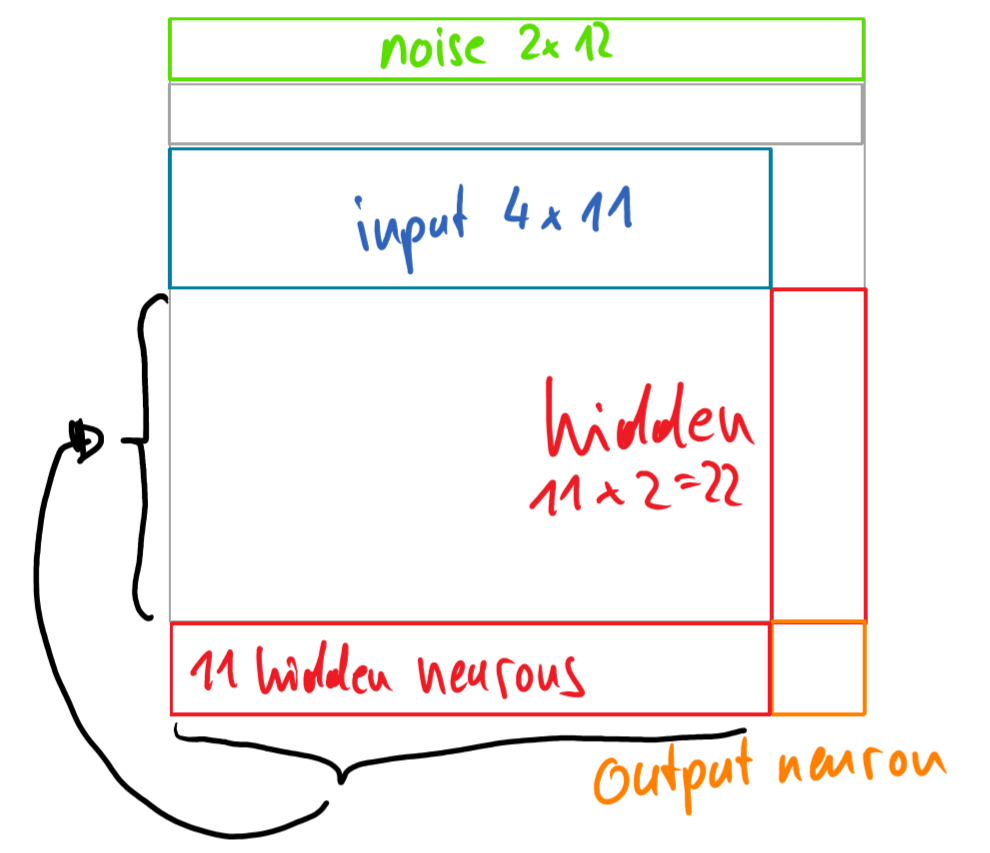
\includegraphics[scale=0.22]{synapse_array_transparent.png}
                \label{membrane_potential}
            \end{figure}
        \endminipage\hfill
    \end{figure}
\end{frame}

% Process
\begin{frame}{Learning Process Step 0/4000} 
	\centering 
	\scalebox{.9}{\begin{tikzpicture} 
	\node (input0) at (2,6.0) {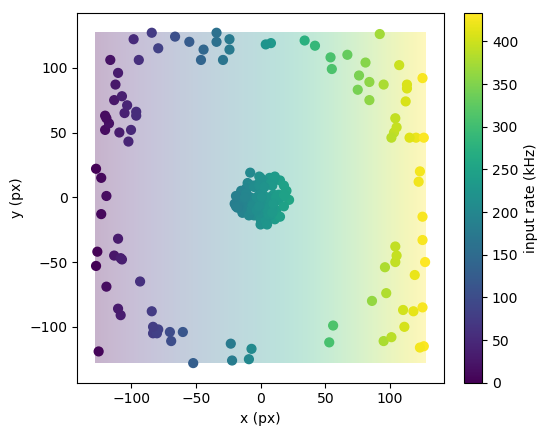
\includegraphics[width=2cm]{learning_process/input_x_map.png}}; 
	\node (input1) at (8,6.0) {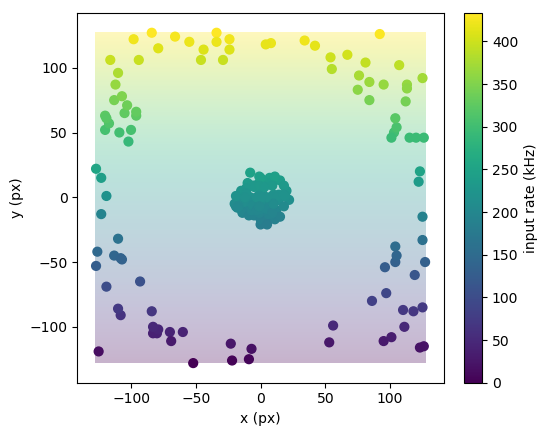
\includegraphics[width=2cm]{learning_process/input_y_map.png}}; 
	\node (hidden0) at (0.0,3.0) {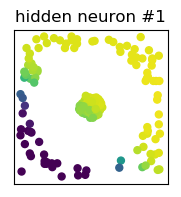
\includegraphics[width=1cm]{learning_process/h_neuron_5_1.png}}; 
	\node (hidden1) at (1.0,3.0) {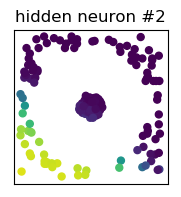
\includegraphics[width=1cm]{learning_process/h_neuron_5_2.png}}; 
	\node (hidden2) at (2.0,3.0) {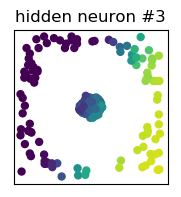
\includegraphics[width=1cm]{learning_process/h_neuron_5_3.png}}; 
	\node (hidden3) at (3.0,3.0) {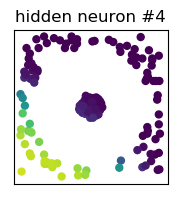
\includegraphics[width=1cm]{learning_process/h_neuron_5_4.png}}; 
	\node (hidden4) at (4.0,3.0) {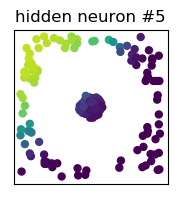
\includegraphics[width=1cm]{learning_process/h_neuron_5_5.png}}; 
	\node (hidden5) at (5.0,3.0) {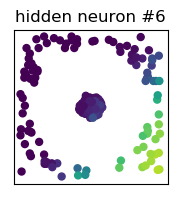
\includegraphics[width=1cm]{learning_process/h_neuron_5_6.png}}; 
	\node (hidden6) at (6.0,3.0) {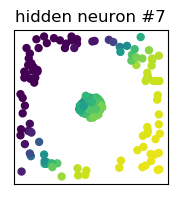
\includegraphics[width=1cm]{learning_process/h_neuron_5_7.png}}; 
	\node (hidden7) at (7.0,3.0) {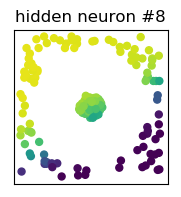
\includegraphics[width=1cm]{learning_process/h_neuron_5_8.png}}; 
	\node (hidden8) at (8.0,3.0) {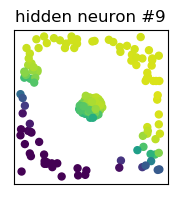
\includegraphics[width=1cm]{learning_process/h_neuron_5_9.png}}; 
	\node (hidden9) at (9.0,3.0) {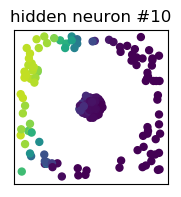
\includegraphics[width=1cm]{learning_process/h_neuron_5_10.png}}; 
	\node (hidden10) at (10.0,3.0) {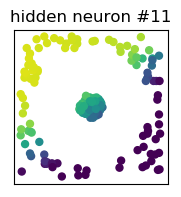
\includegraphics[width=1cm]{learning_process/h_neuron_5_11.png}}; 
 
	\node (out5) at (5.5,0.0) {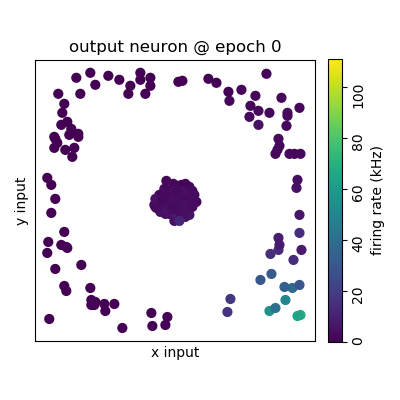
\includegraphics[width=3.6cm]{learning_process/output_neuron_5.png}}; 
	\draw[-stealth,red!100!white,line width=2.1pt] (input0.south) -- (hidden0.north); 
	\draw[-stealth,red!100!white,line width=2.5pt] (input1.south) -- (hidden0.north); 
	\draw[-stealth,blue!100!white,line width=1.3pt] (input0.south) -- (hidden1.north); 
	\draw[-stealth,blue!100!white,line width=2.4pt] (input1.south) -- (hidden1.north); 
	\draw[-stealth,red!100!white,line width=1.5pt] (input0.south) -- (hidden2.north); 
	\draw[-stealth,blue!100!white,line width=0.8pt] (input1.south) -- (hidden2.north); 
	\draw[-stealth,blue!100!white,line width=1.0pt] (input0.south) -- (hidden3.north); 
	\draw[-stealth,blue!100!white,line width=1.4pt] (input1.south) -- (hidden3.north); 
	\draw[-stealth,blue!100!white,line width=1.3pt] (input0.south) -- (hidden4.north); 
	\draw[-stealth,red!100!white,line width=1.6pt] (input1.south) -- (hidden4.north); 
	\draw[-stealth,red!100!white,line width=0.7pt] (input0.south) -- (hidden5.north); 
	\draw[-stealth,blue!100!white,line width=0.7pt] (input1.south) -- (hidden5.north); 
	\draw[-stealth,red!100!white,line width=1.7pt] (input0.south) -- (hidden6.north); 
	\draw[-stealth,blue!100!white,line width=1.2pt] (input1.south) -- (hidden6.north); 
	\draw[-stealth,blue!100!white,line width=1.7pt] (input0.south) -- (hidden7.north); 
	\draw[-stealth,red!100!white,line width=2.8pt] (input1.south) -- (hidden7.north); 
	\draw[-stealth,red!100!white,line width=1.5pt] (input0.south) -- (hidden8.north); 
	\draw[-stealth,red!100!white,line width=2.4pt] (input1.south) -- (hidden8.north); 
	\draw[-stealth,blue!100!white,line width=2.7pt] (input0.south) -- (hidden9.north); 
	\draw[-stealth,red!100!white,line width=1.0pt] (input1.south) -- (hidden9.north); 
	\draw[-stealth,blue!100!white,line width=1.6pt] (input0.south) -- (hidden10.north); 
	\draw[-stealth,red!100!white,line width=2.4pt] (input1.south) -- (hidden10.north); 
	\draw[-stealth,line width=0.4pt, color=red ] (hidden0.south) -- (out5); 
	\draw[-stealth,line width=2.0pt, color=blue ] (hidden1.south) -- (out5); 
	\draw[-stealth,line width=1.9pt, color=red ] (hidden2.south) -- (out5); 
	\draw[-stealth,line width=1.1pt, color=red ] (hidden3.south) -- (out5); 
	\draw[-stealth,line width=2.1pt, color=red ] (hidden4.south) -- (out5); 
	\draw[-stealth,line width=2.2pt, color=red ] (hidden5.south) -- (out5); 
	\draw[-stealth,line width=1.4pt, color=red ] (hidden6.south) -- (out5); 
	\draw[-stealth,line width=0.1pt, color=red ] (hidden7.south) -- (out5); 
	\draw[-stealth,line width=2.2pt, color=blue ] (hidden8.south) -- (out5); 
	\draw[-stealth,line width=0.7pt, color=red ] (hidden9.south) -- (out5); 
	\draw[-stealth,line width=0.7pt, color=red ] (hidden10.south) -- (out5); 
\end{tikzpicture} 
} 
\end{frame} 
\begin{frame}{Learning Process Step 500/4000} 
	\centering 
	\scalebox{.9}{\begin{tikzpicture} 
	\node (input0) at (2,6.0) {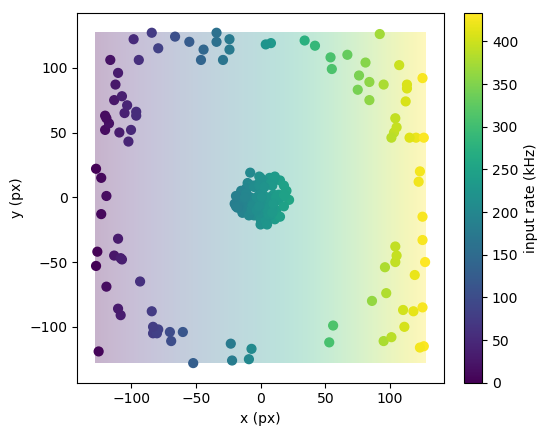
\includegraphics[width=2cm]{learning_process/input_x_map.png}}; 
	\node (input1) at (8,6.0) {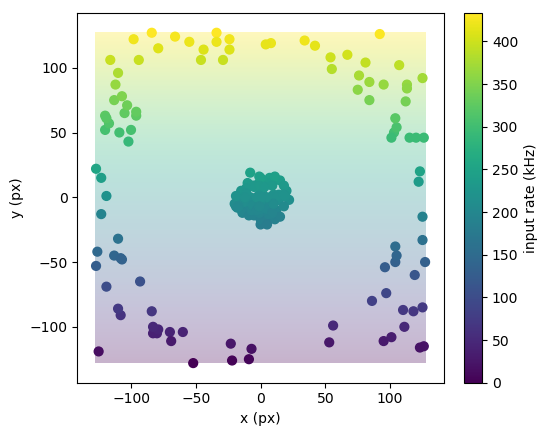
\includegraphics[width=2cm]{learning_process/input_y_map.png}}; 
	\node (hidden0) at (0.0,3.0) {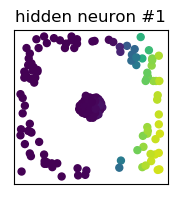
\includegraphics[width=1cm]{learning_process/h_neuron_500_1.png}}; 
	\node (hidden1) at (1.0,3.0) {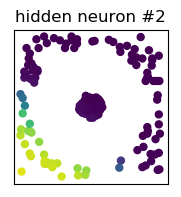
\includegraphics[width=1cm]{learning_process/h_neuron_500_2.png}}; 
	\node (hidden2) at (2.0,3.0) {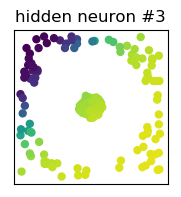
\includegraphics[width=1cm]{learning_process/h_neuron_500_3.png}}; 
	\node (hidden3) at (3.0,3.0) {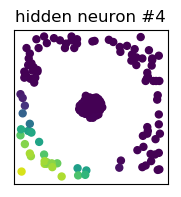
\includegraphics[width=1cm]{learning_process/h_neuron_500_4.png}}; 
	\node (hidden4) at (4.0,3.0) {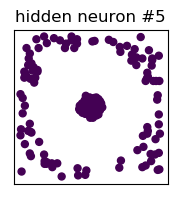
\includegraphics[width=1cm]{learning_process/h_neuron_500_5.png}}; 
	\node (hidden5) at (5.0,3.0) {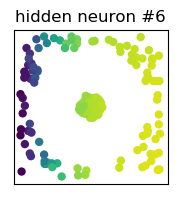
\includegraphics[width=1cm]{learning_process/h_neuron_500_6.png}}; 
	\node (hidden6) at (6.0,3.0) {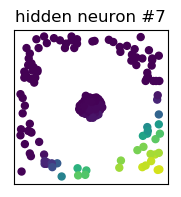
\includegraphics[width=1cm]{learning_process/h_neuron_500_7.png}}; 
	\node (hidden7) at (7.0,3.0) {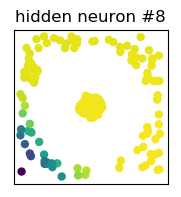
\includegraphics[width=1cm]{learning_process/h_neuron_500_8.png}}; 
	\node (hidden8) at (8.0,3.0) {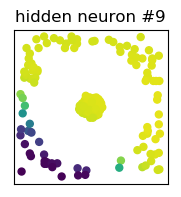
\includegraphics[width=1cm]{learning_process/h_neuron_500_9.png}}; 
	\node (hidden9) at (9.0,3.0) {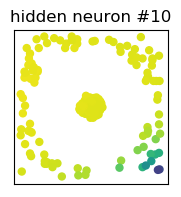
\includegraphics[width=1cm]{learning_process/h_neuron_500_10.png}}; 
	\node (hidden10) at (10.0,3.0) {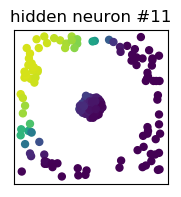
\includegraphics[width=1cm]{learning_process/h_neuron_500_11.png}}; 
 
	\node (out500) at (5.5,0.0) {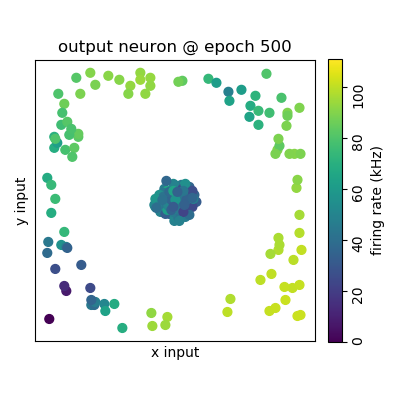
\includegraphics[width=3.6cm]{learning_process/output_neuron_500.png}}; 
	\draw[-stealth,red!100!white,line width=2.2pt] (input0.south) -- (hidden0.north); 
	\draw[-stealth,blue!100!white,line width=0.4pt] (input1.south) -- (hidden0.north); 
	\draw[-stealth,blue!100!white,line width=2.0pt] (input0.south) -- (hidden1.north); 
	\draw[-stealth,blue!100!white,line width=2.8pt] (input1.south) -- (hidden1.north); 
	\draw[-stealth,red!100!white,line width=1.5pt] (input0.south) -- (hidden2.north); 
	\draw[-stealth,blue!100!white,line width=1.2pt] (input1.south) -- (hidden2.north); 
	\draw[-stealth,blue!100!white,line width=1.9pt] (input0.south) -- (hidden3.north); 
	\draw[-stealth,blue!100!white,line width=2.5pt] (input1.south) -- (hidden3.north); 
	\draw[-stealth,red!100!white,line width=0.2pt] (input0.south) -- (hidden4.north); 
	\draw[-stealth,red!100!white,line width=0.1pt] (input1.south) -- (hidden4.north); 
	\draw[-stealth,red!100!white,line width=1.5pt] (input0.south) -- (hidden5.north); 
	\draw[-stealth,gray!100!white,line width=0.0pt] (input1.south) -- (hidden5.north); 
	\draw[-stealth,red!100!white,line width=1.1pt] (input0.south) -- (hidden6.north); 
	\draw[-stealth,blue!100!white,line width=2.1pt] (input1.south) -- (hidden6.north); 
	\draw[-stealth,red!100!white,line width=3.2pt] (input0.south) -- (hidden7.north); 
	\draw[-stealth,red!100!white,line width=2.8pt] (input1.south) -- (hidden7.north); 
	\draw[-stealth,red!100!white,line width=1.9pt] (input0.south) -- (hidden8.north); 
	\draw[-stealth,red!100!white,line width=2.8pt] (input1.south) -- (hidden8.north); 
	\draw[-stealth,blue!100!white,line width=1.1pt] (input0.south) -- (hidden9.north); 
	\draw[-stealth,red!100!white,line width=2.5pt] (input1.south) -- (hidden9.north); 
	\draw[-stealth,blue!100!white,line width=3.1pt] (input0.south) -- (hidden10.north); 
	\draw[-stealth,red!100!white,line width=2.5pt] (input1.south) -- (hidden10.north); 
	\draw[-stealth,line width=1.5pt, color=red ] (hidden0.south) -- (out500); 
	\draw[-stealth,line width=0.1pt, color=blue ] (hidden1.south) -- (out500); 
	\draw[-stealth,line width=0.8pt, color=red ] (hidden2.south) -- (out500); 
	\draw[-stealth,line width=0.7pt, color=red ] (hidden3.south) -- (out500); 
	\draw[-stealth,line width=1.2pt, color=red ] (hidden4.south) -- (out500); 
	\draw[-stealth,line width=2.0pt, color=red ] (hidden5.south) -- (out500); 
	\draw[-stealth,line width=2.3pt, color=red ] (hidden6.south) -- (out500); 
	\draw[-stealth,line width=0.9pt, color=red ] (hidden7.south) -- (out500); 
	\draw[-stealth,line width=0.5pt, color=blue ] (hidden8.south) -- (out500); 
	\draw[-stealth,line width=0.2pt, color=red ] (hidden9.south) -- (out500); 
	\draw[-stealth,line width=2.2pt, color=red ] (hidden10.south) -- (out500); 
\end{tikzpicture} 
} 
\end{frame} 
\begin{frame}{Learning Process Step 1000/4000} 
	\centering 
	\scalebox{.9}{\begin{tikzpicture} 
	\node (input0) at (2,6.0) {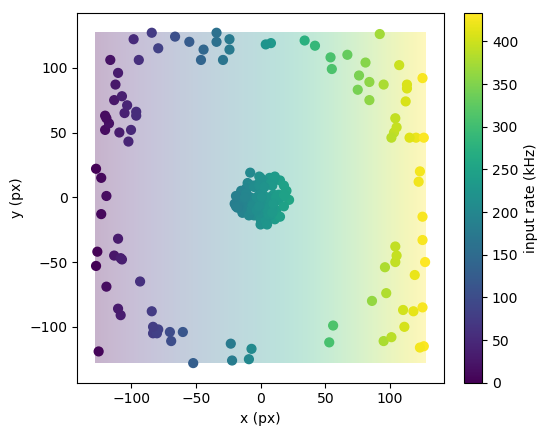
\includegraphics[width=2cm]{learning_process/input_x_map.png}}; 
	\node (input1) at (8,6.0) {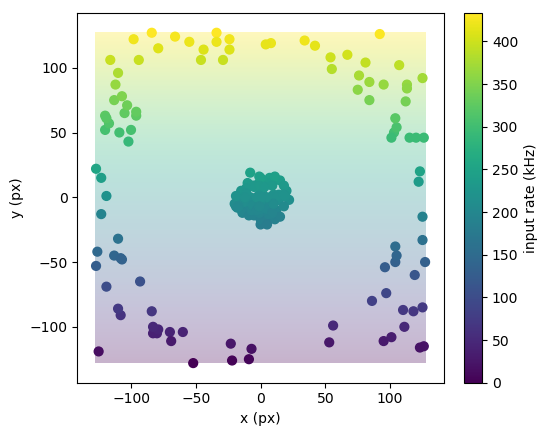
\includegraphics[width=2cm]{learning_process/input_y_map.png}}; 
	\node (hidden0) at (0.0,3.0) {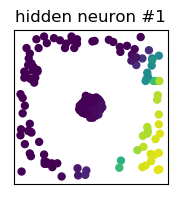
\includegraphics[width=1cm]{learning_process/h_neuron_1000_1.png}}; 
	\node (hidden1) at (1.0,3.0) {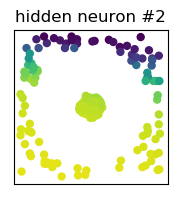
\includegraphics[width=1cm]{learning_process/h_neuron_1000_2.png}}; 
	\node (hidden2) at (2.0,3.0) {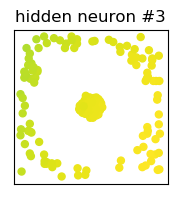
\includegraphics[width=1cm]{learning_process/h_neuron_1000_3.png}}; 
	\node (hidden3) at (3.0,3.0) {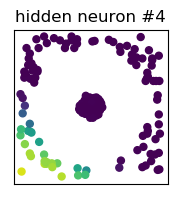
\includegraphics[width=1cm]{learning_process/h_neuron_1000_4.png}}; 
	\node (hidden4) at (4.0,3.0) {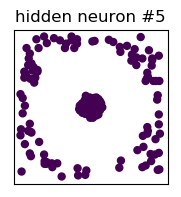
\includegraphics[width=1cm]{learning_process/h_neuron_1000_5.png}}; 
	\node (hidden5) at (5.0,3.0) {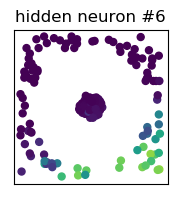
\includegraphics[width=1cm]{learning_process/h_neuron_1000_6.png}}; 
	\node (hidden6) at (6.0,3.0) {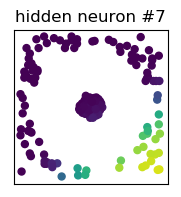
\includegraphics[width=1cm]{learning_process/h_neuron_1000_7.png}}; 
	\node (hidden7) at (7.0,3.0) {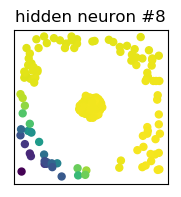
\includegraphics[width=1cm]{learning_process/h_neuron_1000_8.png}}; 
	\node (hidden8) at (8.0,3.0) {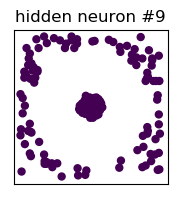
\includegraphics[width=1cm]{learning_process/h_neuron_1000_9.png}}; 
	\node (hidden9) at (9.0,3.0) {\includegraphics[width=1cm]{learning_process/h_neuron_1000_10.png}}; 
	\node (hidden10) at (10.0,3.0) {\includegraphics[width=1cm]{learning_process/h_neuron_1000_11.png}}; 
 
	\node (out1000) at (5.5,0.0) {\includegraphics[width=3.6cm]{learning_process/output_neuron_1000.png}}; 
	\draw[-stealth,red!100!white,line width=2.4pt] (input0.south) -- (hidden0.north); 
	\draw[-stealth,blue!100!white,line width=1.3pt] (input1.south) -- (hidden0.north); 
	\draw[-stealth,blue!100!white,line width=0.4pt] (input0.south) -- (hidden1.north); 
	\draw[-stealth,blue!100!white,line width=1.8pt] (input1.south) -- (hidden1.north); 
	\draw[-stealth,red!100!white,line width=3.1pt] (input0.south) -- (hidden2.north); 
	\draw[-stealth,blue!100!white,line width=0.1pt] (input1.south) -- (hidden2.north); 
	\draw[-stealth,blue!100!white,line width=2.0pt] (input0.south) -- (hidden3.north); 
	\draw[-stealth,blue!100!white,line width=2.7pt] (input1.south) -- (hidden3.north); 
	\draw[-stealth,red!100!white,line width=0.4pt] (input0.south) -- (hidden4.north); 
	\draw[-stealth,red!100!white,line width=0.7pt] (input1.south) -- (hidden4.north); 
	\draw[-stealth,red!100!white,line width=0.3pt] (input0.south) -- (hidden5.north); 
	\draw[-stealth,blue!100!white,line width=1.1pt] (input1.south) -- (hidden5.north); 
	\draw[-stealth,red!100!white,line width=1.3pt] (input0.south) -- (hidden6.north); 
	\draw[-stealth,blue!100!white,line width=1.6pt] (input1.south) -- (hidden6.north); 
	\draw[-stealth,red!100!white,line width=3.2pt] (input0.south) -- (hidden7.north); 
	\draw[-stealth,red!100!white,line width=3.1pt] (input1.south) -- (hidden7.north); 
	\draw[-stealth,red!100!white,line width=1.0pt] (input0.south) -- (hidden8.north); 
	\draw[-stealth,red!100!white,line width=0.2pt] (input1.south) -- (hidden8.north); 
	\draw[-stealth,blue!100!white,line width=0.5pt] (input0.south) -- (hidden9.north); 
	\draw[-stealth,red!100!white,line width=3.2pt] (input1.south) -- (hidden9.north); 
	\draw[-stealth,blue!100!white,line width=2.9pt] (input0.south) -- (hidden10.north); 
	\draw[-stealth,red!100!white,line width=2.4pt] (input1.south) -- (hidden10.north); 
	\draw[-stealth,line width=1.9pt, color=red ] (hidden0.south) -- (out1000); 
	\draw[-stealth,line width=0.0pt, color=blue ] (hidden1.south) -- (out1000); 
	\draw[-stealth,line width=0.7pt, color=red ] (hidden2.south) -- (out1000); 
	\draw[-stealth,line width=1.7pt, color=red ] (hidden3.south) -- (out1000); 
	\draw[-stealth,line width=0.8pt, color=red ] (hidden4.south) -- (out1000); 
	\draw[-stealth,line width=1.3pt, color=red ] (hidden5.south) -- (out1000); 
	\draw[-stealth,line width=2.4pt, color=red ] (hidden6.south) -- (out1000); 
	\draw[-stealth,line width=0.7pt, color=red ] (hidden7.south) -- (out1000); 
	\draw[-stealth,line width=0.3pt, color=blue ] (hidden8.south) -- (out1000); 
	\draw[-stealth,line width=1.1pt, color=red ] (hidden9.south) -- (out1000); 
	\draw[-stealth,line width=1.9pt, color=red ] (hidden10.south) -- (out1000); 
\end{tikzpicture} 
} 
\end{frame} 
\begin{frame}{Learning Process Step 1500/4000} 
	\centering 
	\scalebox{.9}{\begin{tikzpicture} 
	\node (input0) at (2,6.0) {\includegraphics[width=2cm]{learning_process/input_x_map.png}}; 
	\node (input1) at (8,6.0) {\includegraphics[width=2cm]{learning_process/input_y_map.png}}; 
	\node (hidden0) at (0.0,3.0) {\includegraphics[width=1cm]{learning_process/h_neuron_1500_1.png}}; 
	\node (hidden1) at (1.0,3.0) {\includegraphics[width=1cm]{learning_process/h_neuron_1500_2.png}}; 
	\node (hidden2) at (2.0,3.0) {\includegraphics[width=1cm]{learning_process/h_neuron_1500_3.png}}; 
	\node (hidden3) at (3.0,3.0) {\includegraphics[width=1cm]{learning_process/h_neuron_1500_4.png}}; 
	\node (hidden4) at (4.0,3.0) {\includegraphics[width=1cm]{learning_process/h_neuron_1500_5.png}}; 
	\node (hidden5) at (5.0,3.0) {\includegraphics[width=1cm]{learning_process/h_neuron_1500_6.png}}; 
	\node (hidden6) at (6.0,3.0) {\includegraphics[width=1cm]{learning_process/h_neuron_1500_7.png}}; 
	\node (hidden7) at (7.0,3.0) {\includegraphics[width=1cm]{learning_process/h_neuron_1500_8.png}}; 
	\node (hidden8) at (8.0,3.0) {\includegraphics[width=1cm]{learning_process/h_neuron_1500_9.png}}; 
	\node (hidden9) at (9.0,3.0) {\includegraphics[width=1cm]{learning_process/h_neuron_1500_10.png}}; 
	\node (hidden10) at (10.0,3.0) {\includegraphics[width=1cm]{learning_process/h_neuron_1500_11.png}}; 
 
	\node (out1500) at (5.5,0.0) {\includegraphics[width=3.6cm]{learning_process/output_neuron_1500.png}}; 
	\draw[-stealth,red!100!white,line width=2.8pt] (input0.south) -- (hidden0.north); 
	\draw[-stealth,blue!100!white,line width=1.4pt] (input1.south) -- (hidden0.north); 
	\draw[-stealth,blue!100!white,line width=0.6pt] (input0.south) -- (hidden1.north); 
	\draw[-stealth,blue!100!white,line width=2.0pt] (input1.south) -- (hidden1.north); 
	\draw[-stealth,red!100!white,line width=1.5pt] (input0.south) -- (hidden2.north); 
	\draw[-stealth,blue!100!white,line width=1.0pt] (input1.south) -- (hidden2.north); 
	\draw[-stealth,blue!100!white,line width=2.2pt] (input0.south) -- (hidden3.north); 
	\draw[-stealth,blue!100!white,line width=2.7pt] (input1.south) -- (hidden3.north); 
	\draw[-stealth,red!100!white,line width=0.9pt] (input0.south) -- (hidden4.north); 
	\draw[-stealth,red!100!white,line width=1.9pt] (input1.south) -- (hidden4.north); 
	\draw[-stealth,red!100!white,line width=0.4pt] (input0.south) -- (hidden5.north); 
	\draw[-stealth,blue!100!white,line width=1.2pt] (input1.south) -- (hidden5.north); 
	\draw[-stealth,red!100!white,line width=1.0pt] (input0.south) -- (hidden6.north); 
	\draw[-stealth,blue!100!white,line width=2.3pt] (input1.south) -- (hidden6.north); 
	\draw[-stealth,red!100!white,line width=3.1pt] (input0.south) -- (hidden7.north); 
	\draw[-stealth,red!100!white,line width=3.2pt] (input1.south) -- (hidden7.north); 
	\draw[-stealth,red!100!white,line width=0.7pt] (input0.south) -- (hidden8.north); 
	\draw[-stealth,red!100!white,line width=0.2pt] (input1.south) -- (hidden8.north); 
	\draw[-stealth,red!100!white,line width=0.6pt] (input0.south) -- (hidden9.north); 
	\draw[-stealth,red!100!white,line width=1.3pt] (input1.south) -- (hidden9.north); 
	\draw[-stealth,blue!100!white,line width=3.1pt] (input0.south) -- (hidden10.north); 
	\draw[-stealth,red!100!white,line width=2.0pt] (input1.south) -- (hidden10.north); 
	\draw[-stealth,line width=1.8pt, color=red ] (hidden0.south) -- (out1500); 
	\draw[-stealth,line width=0.4pt, color=blue ] (hidden1.south) -- (out1500); 
	\draw[-stealth,line width=0.9pt, color=red ] (hidden2.south) -- (out1500); 
	\draw[-stealth,line width=1.8pt, color=red ] (hidden3.south) -- (out1500); 
	\draw[-stealth,line width=0.4pt, color=red ] (hidden4.south) -- (out1500); 
	\draw[-stealth,line width=1.2pt, color=red ] (hidden5.south) -- (out1500); 
	\draw[-stealth,line width=2.6pt, color=red ] (hidden6.south) -- (out1500); 
	\draw[-stealth,line width=0.1pt, color=red ] (hidden7.south) -- (out1500); 
	\draw[-stealth,line width=0.3pt, color=blue ] (hidden8.south) -- (out1500); 
	\draw[-stealth,line width=2.3pt, color=red ] (hidden9.south) -- (out1500); 
	\draw[-stealth,line width=1.7pt, color=red ] (hidden10.south) -- (out1500); 
\end{tikzpicture} 
} 
\end{frame} 
\begin{frame}{Learning Process Step 2000/4000} 
	\centering 
	\scalebox{.9}{\begin{tikzpicture} 
	\node (input0) at (2,6.0) {\includegraphics[width=2cm]{learning_process/input_x_map.png}}; 
	\node (input1) at (8,6.0) {\includegraphics[width=2cm]{learning_process/input_y_map.png}}; 
	\node (hidden0) at (0.0,3.0) {\includegraphics[width=1cm]{learning_process/h_neuron_2000_1.png}}; 
	\node (hidden1) at (1.0,3.0) {\includegraphics[width=1cm]{learning_process/h_neuron_2000_2.png}}; 
	\node (hidden2) at (2.0,3.0) {\includegraphics[width=1cm]{learning_process/h_neuron_2000_3.png}}; 
	\node (hidden3) at (3.0,3.0) {\includegraphics[width=1cm]{learning_process/h_neuron_2000_4.png}}; 
	\node (hidden4) at (4.0,3.0) {\includegraphics[width=1cm]{learning_process/h_neuron_2000_5.png}}; 
	\node (hidden5) at (5.0,3.0) {\includegraphics[width=1cm]{learning_process/h_neuron_2000_6.png}}; 
	\node (hidden6) at (6.0,3.0) {\includegraphics[width=1cm]{learning_process/h_neuron_2000_7.png}}; 
	\node (hidden7) at (7.0,3.0) {\includegraphics[width=1cm]{learning_process/h_neuron_2000_8.png}}; 
	\node (hidden8) at (8.0,3.0) {\includegraphics[width=1cm]{learning_process/h_neuron_2000_9.png}}; 
	\node (hidden9) at (9.0,3.0) {\includegraphics[width=1cm]{learning_process/h_neuron_2000_10.png}}; 
	\node (hidden10) at (10.0,3.0) {\includegraphics[width=1cm]{learning_process/h_neuron_2000_11.png}}; 
 
	\node (out2000) at (5.5,0.0) {\includegraphics[width=3.6cm]{learning_process/output_neuron_2000.png}}; 
	\draw[-stealth,red!100!white,line width=3.1pt] (input0.south) -- (hidden0.north); 
	\draw[-stealth,blue!100!white,line width=0.4pt] (input1.south) -- (hidden0.north); 
	\draw[-stealth,red!100!white,line width=0.1pt] (input0.south) -- (hidden1.north); 
	\draw[-stealth,blue!100!white,line width=3.2pt] (input1.south) -- (hidden1.north); 
	\draw[-stealth,red!100!white,line width=0.1pt] (input0.south) -- (hidden2.north); 
	\draw[-stealth,blue!100!white,line width=1.3pt] (input1.south) -- (hidden2.north); 
	\draw[-stealth,blue!100!white,line width=2.2pt] (input0.south) -- (hidden3.north); 
	\draw[-stealth,blue!100!white,line width=2.7pt] (input1.south) -- (hidden3.north); 
	\draw[-stealth,red!100!white,line width=0.4pt] (input0.south) -- (hidden4.north); 
	\draw[-stealth,red!100!white,line width=3.3pt] (input1.south) -- (hidden4.north); 
	\draw[-stealth,red!100!white,line width=0.1pt] (input0.south) -- (hidden5.north); 
	\draw[-stealth,blue!100!white,line width=1.3pt] (input1.south) -- (hidden5.north); 
	\draw[-stealth,red!100!white,line width=1.4pt] (input0.south) -- (hidden6.north); 
	\draw[-stealth,blue!100!white,line width=1.7pt] (input1.south) -- (hidden6.north); 
	\draw[-stealth,red!100!white,line width=3.1pt] (input0.south) -- (hidden7.north); 
	\draw[-stealth,red!100!white,line width=3.2pt] (input1.south) -- (hidden7.north); 
	\draw[-stealth,red!100!white,line width=0.6pt] (input0.south) -- (hidden8.north); 
	\draw[-stealth,red!100!white,line width=0.2pt] (input1.south) -- (hidden8.north); 
	\draw[-stealth,blue!100!white,line width=1.3pt] (input0.south) -- (hidden9.north); 
	\draw[-stealth,red!100!white,line width=0.7pt] (input1.south) -- (hidden9.north); 
	\draw[-stealth,blue!100!white,line width=3.1pt] (input0.south) -- (hidden10.north); 
	\draw[-stealth,red!100!white,line width=2.1pt] (input1.south) -- (hidden10.north); 
	\draw[-stealth,line width=1.9pt, color=red ] (hidden0.south) -- (out2000); 
	\draw[-stealth,line width=1.5pt, color=blue ] (hidden1.south) -- (out2000); 
	\draw[-stealth,line width=0.6pt, color=red ] (hidden2.south) -- (out2000); 
	\draw[-stealth,line width=1.9pt, color=red ] (hidden3.south) -- (out2000); 
	\draw[-stealth,line width=0.2pt, color=red ] (hidden4.south) -- (out2000); 
	\draw[-stealth,line width=1.2pt, color=red ] (hidden5.south) -- (out2000); 
	\draw[-stealth,line width=2.4pt, color=red ] (hidden6.south) -- (out2000); 
	\draw[-stealth,line width=0.1pt, color=red ] (hidden7.south) -- (out2000); 
	\draw[-stealth,line width=0.3pt, color=blue ] (hidden8.south) -- (out2000); 
	\draw[-stealth,line width=2.4pt, color=red ] (hidden9.south) -- (out2000); 
	\draw[-stealth,line width=1.7pt, color=red ] (hidden10.south) -- (out2000); 
\end{tikzpicture} 
} 
\end{frame} 
\begin{frame}{Learning Process Step 2500/4000} 
	\centering 
	\scalebox{.9}{\begin{tikzpicture} 
	\node (input0) at (2,6.0) {\includegraphics[width=2cm]{learning_process/input_x_map.png}}; 
	\node (input1) at (8,6.0) {\includegraphics[width=2cm]{learning_process/input_y_map.png}}; 
	\node (hidden0) at (0.0,3.0) {\includegraphics[width=1cm]{learning_process/h_neuron_2500_1.png}}; 
	\node (hidden1) at (1.0,3.0) {\includegraphics[width=1cm]{learning_process/h_neuron_2500_2.png}}; 
	\node (hidden2) at (2.0,3.0) {\includegraphics[width=1cm]{learning_process/h_neuron_2500_3.png}}; 
	\node (hidden3) at (3.0,3.0) {\includegraphics[width=1cm]{learning_process/h_neuron_2500_4.png}}; 
	\node (hidden4) at (4.0,3.0) {\includegraphics[width=1cm]{learning_process/h_neuron_2500_5.png}}; 
	\node (hidden5) at (5.0,3.0) {\includegraphics[width=1cm]{learning_process/h_neuron_2500_6.png}}; 
	\node (hidden6) at (6.0,3.0) {\includegraphics[width=1cm]{learning_process/h_neuron_2500_7.png}}; 
	\node (hidden7) at (7.0,3.0) {\includegraphics[width=1cm]{learning_process/h_neuron_2500_8.png}}; 
	\node (hidden8) at (8.0,3.0) {\includegraphics[width=1cm]{learning_process/h_neuron_2500_9.png}}; 
	\node (hidden9) at (9.0,3.0) {\includegraphics[width=1cm]{learning_process/h_neuron_2500_10.png}}; 
	\node (hidden10) at (10.0,3.0) {\includegraphics[width=1cm]{learning_process/h_neuron_2500_11.png}}; 
 
	\node (out2500) at (5.5,0.0) {\includegraphics[width=3.6cm]{learning_process/output_neuron_2500.png}}; 
	\draw[-stealth,red!100!white,line width=2.5pt] (input0.south) -- (hidden0.north); 
	\draw[-stealth,red!100!white,line width=0.2pt] (input1.south) -- (hidden0.north); 
	\draw[-stealth,gray!100!white,line width=0.0pt] (input0.south) -- (hidden1.north); 
	\draw[-stealth,blue!100!white,line width=3.1pt] (input1.south) -- (hidden1.north); 
	\draw[-stealth,blue!100!white,line width=1.4pt] (input0.south) -- (hidden2.north); 
	\draw[-stealth,blue!100!white,line width=2.1pt] (input1.south) -- (hidden2.north); 
	\draw[-stealth,blue!100!white,line width=2.4pt] (input0.south) -- (hidden3.north); 
	\draw[-stealth,blue!100!white,line width=2.8pt] (input1.south) -- (hidden3.north); 
	\draw[-stealth,red!100!white,line width=3.0pt] (input0.south) -- (hidden4.north); 
	\draw[-stealth,red!100!white,line width=3.2pt] (input1.south) -- (hidden4.north); 
	\draw[-stealth,gray!100!white,line width=0.0pt] (input0.south) -- (hidden5.north); 
	\draw[-stealth,blue!100!white,line width=1.2pt] (input1.south) -- (hidden5.north); 
	\draw[-stealth,red!100!white,line width=1.8pt] (input0.south) -- (hidden6.north); 
	\draw[-stealth,blue!100!white,line width=2.5pt] (input1.south) -- (hidden6.north); 
	\draw[-stealth,red!100!white,line width=3.1pt] (input0.south) -- (hidden7.north); 
	\draw[-stealth,red!100!white,line width=3.1pt] (input1.south) -- (hidden7.north); 
	\draw[-stealth,red!100!white,line width=0.6pt] (input0.south) -- (hidden8.north); 
	\draw[-stealth,red!100!white,line width=0.3pt] (input1.south) -- (hidden8.north); 
	\draw[-stealth,blue!100!white,line width=3.1pt] (input0.south) -- (hidden9.north); 
	\draw[-stealth,blue!100!white,line width=1.0pt] (input1.south) -- (hidden9.north); 
	\draw[-stealth,blue!100!white,line width=2.5pt] (input0.south) -- (hidden10.north); 
	\draw[-stealth,red!100!white,line width=2.0pt] (input1.south) -- (hidden10.north); 
	\draw[-stealth,line width=2.5pt, color=red ] (hidden0.south) -- (out2500); 
	\draw[-stealth,line width=1.9pt, color=blue ] (hidden1.south) -- (out2500); 
	\draw[-stealth,line width=0.1pt, color=red ] (hidden2.south) -- (out2500); 
	\draw[-stealth,line width=2.1pt, color=red ] (hidden3.south) -- (out2500); 
	\draw[-stealth,line width=1.2pt, color=red ] (hidden4.south) -- (out2500); 
	\draw[-stealth,line width=1.2pt, color=red ] (hidden5.south) -- (out2500); 
	\draw[-stealth,line width=2.6pt, color=red ] (hidden6.south) -- (out2500); 
	\draw[-stealth,line width=0.7pt, color=red ] (hidden7.south) -- (out2500); 
	\draw[-stealth,line width=0.3pt, color=blue ] (hidden8.south) -- (out2500); 
	\draw[-stealth,line width=2.5pt, color=red ] (hidden9.south) -- (out2500); 
	\draw[-stealth,line width=1.7pt, color=red ] (hidden10.south) -- (out2500); 
\end{tikzpicture} 
} 
\end{frame} 
\begin{frame}{Learning Process Step 3000/4000} 
	\centering 
	\scalebox{.9}{\begin{tikzpicture} 
	\node (input0) at (2,6.0) {\includegraphics[width=2cm]{learning_process/input_x_map.png}}; 
	\node (input1) at (8,6.0) {\includegraphics[width=2cm]{learning_process/input_y_map.png}}; 
	\node (hidden0) at (0.0,3.0) {\includegraphics[width=1cm]{learning_process/h_neuron_3000_1.png}}; 
	\node (hidden1) at (1.0,3.0) {\includegraphics[width=1cm]{learning_process/h_neuron_3000_2.png}}; 
	\node (hidden2) at (2.0,3.0) {\includegraphics[width=1cm]{learning_process/h_neuron_3000_3.png}}; 
	\node (hidden3) at (3.0,3.0) {\includegraphics[width=1cm]{learning_process/h_neuron_3000_4.png}}; 
	\node (hidden4) at (4.0,3.0) {\includegraphics[width=1cm]{learning_process/h_neuron_3000_5.png}}; 
	\node (hidden5) at (5.0,3.0) {\includegraphics[width=1cm]{learning_process/h_neuron_3000_6.png}}; 
	\node (hidden6) at (6.0,3.0) {\includegraphics[width=1cm]{learning_process/h_neuron_3000_7.png}}; 
	\node (hidden7) at (7.0,3.0) {\includegraphics[width=1cm]{learning_process/h_neuron_3000_8.png}}; 
	\node (hidden8) at (8.0,3.0) {\includegraphics[width=1cm]{learning_process/h_neuron_3000_9.png}}; 
	\node (hidden9) at (9.0,3.0) {\includegraphics[width=1cm]{learning_process/h_neuron_3000_10.png}}; 
	\node (hidden10) at (10.0,3.0) {\includegraphics[width=1cm]{learning_process/h_neuron_3000_11.png}}; 
 
	\node (out3000) at (5.5,0.0) {\includegraphics[width=3.6cm]{learning_process/output_neuron_3000.png}}; 
	\draw[-stealth,red!100!white,line width=2.4pt] (input0.south) -- (hidden0.north); 
	\draw[-stealth,red!100!white,line width=0.2pt] (input1.south) -- (hidden0.north); 
	\draw[-stealth,red!100!white,line width=0.3pt] (input0.south) -- (hidden1.north); 
	\draw[-stealth,blue!100!white,line width=2.6pt] (input1.south) -- (hidden1.north); 
	\draw[-stealth,blue!100!white,line width=2.0pt] (input0.south) -- (hidden2.north); 
	\draw[-stealth,blue!100!white,line width=2.2pt] (input1.south) -- (hidden2.north); 
	\draw[-stealth,blue!100!white,line width=2.5pt] (input0.south) -- (hidden3.north); 
	\draw[-stealth,blue!100!white,line width=2.8pt] (input1.south) -- (hidden3.north); 
	\draw[-stealth,red!100!white,line width=2.8pt] (input0.south) -- (hidden4.north); 
	\draw[-stealth,red!100!white,line width=2.9pt] (input1.south) -- (hidden4.north); 
	\draw[-stealth,gray!100!white,line width=0.0pt] (input0.south) -- (hidden5.north); 
	\draw[-stealth,blue!100!white,line width=1.2pt] (input1.south) -- (hidden5.north); 
	\draw[-stealth,red!100!white,line width=1.3pt] (input0.south) -- (hidden6.north); 
	\draw[-stealth,blue!100!white,line width=2.2pt] (input1.south) -- (hidden6.north); 
	\draw[-stealth,red!100!white,line width=2.5pt] (input0.south) -- (hidden7.north); 
	\draw[-stealth,red!100!white,line width=3.0pt] (input1.south) -- (hidden7.north); 
	\draw[-stealth,red!100!white,line width=0.6pt] (input0.south) -- (hidden8.north); 
	\draw[-stealth,red!100!white,line width=0.1pt] (input1.south) -- (hidden8.north); 
	\draw[-stealth,blue!100!white,line width=3.1pt] (input0.south) -- (hidden9.north); 
	\draw[-stealth,blue!100!white,line width=0.8pt] (input1.south) -- (hidden9.north); 
	\draw[-stealth,blue!100!white,line width=2.8pt] (input0.south) -- (hidden10.north); 
	\draw[-stealth,red!100!white,line width=1.5pt] (input1.south) -- (hidden10.north); 
	\draw[-stealth,line width=2.4pt, color=red ] (hidden0.south) -- (out3000); 
	\draw[-stealth,line width=2.0pt, color=blue ] (hidden1.south) -- (out3000); 
	\draw[-stealth,line width=0.0pt, color=red ] (hidden2.south) -- (out3000); 
	\draw[-stealth,line width=2.1pt, color=red ] (hidden3.south) -- (out3000); 
	\draw[-stealth,line width=1.3pt, color=red ] (hidden4.south) -- (out3000); 
	\draw[-stealth,line width=1.2pt, color=red ] (hidden5.south) -- (out3000); 
	\draw[-stealth,line width=2.6pt, color=red ] (hidden6.south) -- (out3000); 
	\draw[-stealth,line width=0.7pt, color=red ] (hidden7.south) -- (out3000); 
	\draw[-stealth,line width=0.3pt, color=blue ] (hidden8.south) -- (out3000); 
	\draw[-stealth,line width=2.5pt, color=red ] (hidden9.south) -- (out3000); 
	\draw[-stealth,line width=1.7pt, color=red ] (hidden10.south) -- (out3000); 
\end{tikzpicture} 
} 
\end{frame} 
\begin{frame}{Learning Process Step 3500/4000} 
	\centering 
	\scalebox{.9}{\begin{tikzpicture} 
	\node (input0) at (2,6.0) {\includegraphics[width=2cm]{learning_process/input_x_map.png}}; 
	\node (input1) at (8,6.0) {\includegraphics[width=2cm]{learning_process/input_y_map.png}}; 
	\node (hidden0) at (0.0,3.0) {\includegraphics[width=1cm]{learning_process/h_neuron_3500_1.png}}; 
	\node (hidden1) at (1.0,3.0) {\includegraphics[width=1cm]{learning_process/h_neuron_3500_2.png}}; 
	\node (hidden2) at (2.0,3.0) {\includegraphics[width=1cm]{learning_process/h_neuron_3500_3.png}}; 
	\node (hidden3) at (3.0,3.0) {\includegraphics[width=1cm]{learning_process/h_neuron_3500_4.png}}; 
	\node (hidden4) at (4.0,3.0) {\includegraphics[width=1cm]{learning_process/h_neuron_3500_5.png}}; 
	\node (hidden5) at (5.0,3.0) {\includegraphics[width=1cm]{learning_process/h_neuron_3500_6.png}}; 
	\node (hidden6) at (6.0,3.0) {\includegraphics[width=1cm]{learning_process/h_neuron_3500_7.png}}; 
	\node (hidden7) at (7.0,3.0) {\includegraphics[width=1cm]{learning_process/h_neuron_3500_8.png}}; 
	\node (hidden8) at (8.0,3.0) {\includegraphics[width=1cm]{learning_process/h_neuron_3500_9.png}}; 
	\node (hidden9) at (9.0,3.0) {\includegraphics[width=1cm]{learning_process/h_neuron_3500_10.png}}; 
	\node (hidden10) at (10.0,3.0) {\includegraphics[width=1cm]{learning_process/h_neuron_3500_11.png}}; 
 
	\node (out3500) at (5.5,0.0) {\includegraphics[width=3.6cm]{learning_process/output_neuron_3500.png}}; 
	\draw[-stealth,red!100!white,line width=2.7pt] (input0.south) -- (hidden0.north); 
	\draw[-stealth,red!100!white,line width=0.1pt] (input1.south) -- (hidden0.north); 
	\draw[-stealth,blue!100!white,line width=0.2pt] (input0.south) -- (hidden1.north); 
	\draw[-stealth,blue!100!white,line width=3.1pt] (input1.south) -- (hidden1.north); 
	\draw[-stealth,blue!100!white,line width=2.6pt] (input0.south) -- (hidden2.north); 
	\draw[-stealth,blue!100!white,line width=2.6pt] (input1.south) -- (hidden2.north); 
	\draw[-stealth,blue!100!white,line width=2.6pt] (input0.south) -- (hidden3.north); 
	\draw[-stealth,blue!100!white,line width=2.8pt] (input1.south) -- (hidden3.north); 
	\draw[-stealth,red!100!white,line width=2.6pt] (input0.south) -- (hidden4.north); 
	\draw[-stealth,red!100!white,line width=2.8pt] (input1.south) -- (hidden4.north); 
	\draw[-stealth,gray!100!white,line width=0.0pt] (input0.south) -- (hidden5.north); 
	\draw[-stealth,blue!100!white,line width=1.2pt] (input1.south) -- (hidden5.north); 
	\draw[-stealth,red!100!white,line width=1.3pt] (input0.south) -- (hidden6.north); 
	\draw[-stealth,blue!100!white,line width=2.5pt] (input1.south) -- (hidden6.north); 
	\draw[-stealth,red!100!white,line width=3.0pt] (input0.south) -- (hidden7.north); 
	\draw[-stealth,red!100!white,line width=2.8pt] (input1.south) -- (hidden7.north); 
	\draw[-stealth,red!100!white,line width=0.5pt] (input0.south) -- (hidden8.north); 
	\draw[-stealth,red!100!white,line width=0.2pt] (input1.south) -- (hidden8.north); 
	\draw[-stealth,blue!100!white,line width=3.1pt] (input0.south) -- (hidden9.north); 
	\draw[-stealth,blue!100!white,line width=0.8pt] (input1.south) -- (hidden9.north); 
	\draw[-stealth,blue!100!white,line width=2.4pt] (input0.south) -- (hidden10.north); 
	\draw[-stealth,red!100!white,line width=1.7pt] (input1.south) -- (hidden10.north); 
	\draw[-stealth,line width=2.3pt, color=red ] (hidden0.south) -- (out3500); 
	\draw[-stealth,line width=2.0pt, color=blue ] (hidden1.south) -- (out3500); 
	\draw[-stealth,line width=0.1pt, color=red ] (hidden2.south) -- (out3500); 
	\draw[-stealth,line width=2.1pt, color=red ] (hidden3.south) -- (out3500); 
	\draw[-stealth,line width=1.3pt, color=red ] (hidden4.south) -- (out3500); 
	\draw[-stealth,line width=1.2pt, color=red ] (hidden5.south) -- (out3500); 
	\draw[-stealth,line width=2.3pt, color=red ] (hidden6.south) -- (out3500); 
	\draw[-stealth,line width=0.7pt, color=red ] (hidden7.south) -- (out3500); 
	\draw[-stealth,line width=0.3pt, color=blue ] (hidden8.south) -- (out3500); 
	\draw[-stealth,line width=2.5pt, color=red ] (hidden9.south) -- (out3500); 
	\draw[-stealth,line width=1.5pt, color=red ] (hidden10.south) -- (out3500); 
\end{tikzpicture} 
} 
\end{frame} 
\begin{frame}{Learning Process Step 4000/4000} 
	\centering 
	\scalebox{.9}{\begin{tikzpicture} 
	\node (input0) at (2,6.0) {\includegraphics[width=2cm]{learning_process/input_x_map.png}}; 
	\node (input1) at (8,6.0) {\includegraphics[width=2cm]{learning_process/input_y_map.png}}; 
	\node (hidden0) at (0.0,3.0) {\includegraphics[width=1cm]{learning_process/h_neuron_4000_1.png}}; 
	\node (hidden1) at (1.0,3.0) {\includegraphics[width=1cm]{learning_process/h_neuron_4000_2.png}}; 
	\node (hidden2) at (2.0,3.0) {\includegraphics[width=1cm]{learning_process/h_neuron_4000_3.png}}; 
	\node (hidden3) at (3.0,3.0) {\includegraphics[width=1cm]{learning_process/h_neuron_4000_4.png}}; 
	\node (hidden4) at (4.0,3.0) {\includegraphics[width=1cm]{learning_process/h_neuron_4000_5.png}}; 
	\node (hidden5) at (5.0,3.0) {\includegraphics[width=1cm]{learning_process/h_neuron_4000_6.png}}; 
	\node (hidden6) at (6.0,3.0) {\includegraphics[width=1cm]{learning_process/h_neuron_4000_7.png}}; 
	\node (hidden7) at (7.0,3.0) {\includegraphics[width=1cm]{learning_process/h_neuron_4000_8.png}}; 
	\node (hidden8) at (8.0,3.0) {\includegraphics[width=1cm]{learning_process/h_neuron_4000_9.png}}; 
	\node (hidden9) at (9.0,3.0) {\includegraphics[width=1cm]{learning_process/h_neuron_4000_10.png}}; 
	\node (hidden10) at (10.0,3.0) {\includegraphics[width=1cm]{learning_process/h_neuron_4000_11.png}}; 
 
	\node (out4000) at (5.5,0.0) {\includegraphics[width=3.6cm]{learning_process/output_neuron_4000.png}}; 
	\draw[-stealth,red!100!white,line width=2.6pt] (input0.south) -- (hidden0.north); 
	\draw[-stealth,red!100!white,line width=0.1pt] (input1.south) -- (hidden0.north); 
	\draw[-stealth,blue!100!white,line width=0.5pt] (input0.south) -- (hidden1.north); 
	\draw[-stealth,blue!100!white,line width=3.1pt] (input1.south) -- (hidden1.north); 
	\draw[-stealth,blue!100!white,line width=2.9pt] (input0.south) -- (hidden2.north); 
	\draw[-stealth,blue!100!white,line width=3.1pt] (input1.south) -- (hidden2.north); 
	\draw[-stealth,blue!100!white,line width=2.8pt] (input0.south) -- (hidden3.north); 
	\draw[-stealth,blue!100!white,line width=2.8pt] (input1.south) -- (hidden3.north); 
	\draw[-stealth,red!100!white,line width=2.7pt] (input0.south) -- (hidden4.north); 
	\draw[-stealth,red!100!white,line width=3.3pt] (input1.south) -- (hidden4.north); 
	\draw[-stealth,gray!100!white,line width=0.0pt] (input0.south) -- (hidden5.north); 
	\draw[-stealth,blue!100!white,line width=1.2pt] (input1.south) -- (hidden5.north); 
	\draw[-stealth,red!100!white,line width=1.7pt] (input0.south) -- (hidden6.north); 
	\draw[-stealth,blue!100!white,line width=3.1pt] (input1.south) -- (hidden6.north); 
	\draw[-stealth,red!100!white,line width=3.1pt] (input0.south) -- (hidden7.north); 
	\draw[-stealth,red!100!white,line width=3.3pt] (input1.south) -- (hidden7.north); 
	\draw[-stealth,red!100!white,line width=0.7pt] (input0.south) -- (hidden8.north); 
	\draw[-stealth,red!100!white,line width=0.2pt] (input1.south) -- (hidden8.north); 
	\draw[-stealth,blue!100!white,line width=3.1pt] (input0.south) -- (hidden9.north); 
	\draw[-stealth,blue!100!white,line width=2.8pt] (input1.south) -- (hidden9.north); 
	\draw[-stealth,blue!100!white,line width=2.7pt] (input0.south) -- (hidden10.north); 
	\draw[-stealth,red!100!white,line width=1.8pt] (input1.south) -- (hidden10.north); 
	\draw[-stealth,line width=2.2pt, color=red ] (hidden0.south) -- (out4000); 
	\draw[-stealth,line width=2.0pt, color=blue ] (hidden1.south) -- (out4000); 
	\draw[-stealth,line width=0.1pt, color=red ] (hidden2.south) -- (out4000); 
	\draw[-stealth,line width=2.2pt, color=red ] (hidden3.south) -- (out4000); 
	\draw[-stealth,line width=1.3pt, color=red ] (hidden4.south) -- (out4000); 
	\draw[-stealth,line width=1.2pt, color=red ] (hidden5.south) -- (out4000); 
	\draw[-stealth,line width=2.3pt, color=red ] (hidden6.south) -- (out4000); 
	\draw[-stealth,line width=0.6pt, color=red ] (hidden7.south) -- (out4000); 
	\draw[-stealth,line width=0.3pt, color=blue ] (hidden8.south) -- (out4000); 
	\draw[-stealth,line width=2.5pt, color=red ] (hidden9.south) -- (out4000); 
	\draw[-stealth,line width=2.0pt, color=red ] (hidden10.south) -- (out4000); 
\end{tikzpicture} 
} 
\end{frame} 

% Performance
\begin{frame}{Learning Performance}
\begin{figure}[!htb]
	\minipage{0.65\textwidth}
        \begin{figure}
            \includegraphics[scale=0.6]{learning_process/learning_performance.png}
        \end{figure}
  	\endminipage\hfill
  	\minipage{0.35\textwidth}
  	\centering
        target
        \begin{figure}
            \includegraphics[scale=0.25]{targets.png}
            \label{fig:my_label}
        \end{figure}
        output
        \begin{figure}
            \includegraphics[scale=0.25]{output_neuron_4000.png}
            \label{fig:my_label}
        \end{figure}
    \endminipage\hfill
\end{figure}
\end{frame}

\section[Summary]{Summary}

\begin{frame}{Conclusion and Outlook}
\begin{figure}[!htb]
	\minipage{0.7\textwidth}
        \textbf{Circles}
            \begin{itemize}
                \item performance with shorter measurement period
                \item controlled decalibration
                \item stability: better choice of system parameters
                \item implementation on HICANN-X
            \end{itemize}
        \textbf{SuperSpike}
        \begin{itemize}
            \item prototype implementation on HICANN-X (computation via host)
            \item implement host computation on-chip
            \item on-chip only possible with next tape-out (Spring 2020)
        \end{itemize}
  	\endminipage\hfill
  	\minipage{0.3\textwidth}
  	\centering
        \begin{figure}
            \includegraphics[scale=0.3]{output_neuron_4000.png}
            \label{fig:my_label}
        \end{figure}
    \endminipage\hfill
\end{figure}
\end{frame}

\appendix

\begin{frame}[fragile]{Backup slides}
\centering
        \begin{figure}
            \includegraphics[scale=0.5]{model_parameters.png}
            \label{fig:my_label}
        \end{figure}
\end{frame}

\begin{frame}[fragile]{Backup slides}
\centering
        \begin{figure}
            \includegraphics[scale=0.65]{rates_dist.png}
            \label{fig:my_label}
        \end{figure}
\end{frame}

\begin{frame}[fragile]{Backup slides}
\textbf{Hardware Parameters}
\begin{itemize}
    \item $\tau_{\text{syn\_exc}}$ = 1e-5 s
    \item $\tau_{\text{mem}}$ = 5e-7 s
    \item $\tau_{\text{refrac}}$ = 9e-6 s
    \item PulseLength = 1
    \item Mmnt periode = 2.3 ms
\end{itemize}
\end{frame}
  	
\end{document}